
\documentclass[9pt]{beamer}
%\makeatletter
%\def\beamer@calltheme#1#2#3{%
%	\def\beamer@themelist{#2}
%	\@for\beamer@themename:=\beamer@themelist\do
%	{\usepackage[{#1}]{\beamer@themelocation/#3\beamer@themename}}}
%
%\def\usefolder#1{
%	\def\beamer@themelocation{#1}
%}
%\def\beamer@themelocation{}

%\usefolder{../config}

\usetheme[
block=fill,
titleformat=regular,
progressbar=frametitle
]{metropolis}
%\metroset[everytitleformat=regular] % regular, lowercase, uppercase ]
%\metroset[inner/block=fill]

%\setbeameroption{show notes} 
\usepackage{booktabs}
\usepackage[scale=2]{ccicons}

\usepackage{pgfplots}
\usepgfplotslibrary{dateplot}


%\ Hrvatski znakovi
\usepackage[utf8]{inputenc}
\usepackage[T1]{fontenc}
\usepackage[croatian]{babel}
\usepackage{todonotes}
\usepackage{amsmath}
\usepackage{amsfonts}
\selectlanguage{croatian} % american ngerman
\usepackage{todonotes}

% Koristenje Latin modern fonta
% Bez toga na nekim racunalima baca
% err: Font <taj i taj> at <mala velicina, npr4.0pt> not loadable: Metric (TFM) file not found. \end{frame}
\usepackage{lmodern}


\definecolor{RoyalBlue}{cmyk}{1, 0.50, 0, 0}
%\usepackage{natbib}
%\usepackage{bibentry}
\usepackage{scrextend}
\usepackage{hyperref}
%\usepackage[pdfa=true]{hyperref}
\hypersetup{%
    %draft, % = no hyperlinking at all (useful in b/w printouts)
    %colorlinks=true, 
    linktocpage=true, pdfstartpage=3, pdfstartview=FitV,%
    % uncomment the following line if you want to have black links (e.g., for printing)
    %colorlinks=false, linktocpage=false, pdfborder={0 0 0}, pdfstartpage=3, pdfstartview=FitV,% 
    breaklinks=true, pdfpagemode=UseNone, pageanchor=true, pdfpagemode=UseOutlines,%
    plainpages=false, bookmarksnumbered, bookmarksopen=true, bookmarksopenlevel=1,%
    hypertexnames=true, pdfhighlight=/O,%nesting=true,%frenchlinks,%
    %urlcolor=webbrown, linkcolor=RoyalBlue, citecolor=webgreen, %pagecolor=RoyalBlue,%
    %urlcolor=Blue, linkcolor=Blue, citecolor=Red, %pagecolor=Black,%
    %pdftitle={\myTitle},%
    %pdfauthor={\textcopyright\ \myName, \myUni, \myFaculty},%
    pdfsubject={},%
    pdfkeywords={},%
    pdfcreator={pdfLaTeX},%
    pdfproducer={LaTeX with hyperref and classicthesis}, %
    unicode = true 
} 

%\usepackage[pdftex]{graphicx}
% declare the path(s) where your graphic files are
\graphicspath{{./}{./figures/}}


\newcommand{\executeiffilenewer}[3]{%
	\ifnum\pdfstrcmp{\pdffilemoddate{#1}}%
	{\pdffilemoddate{#2}}>0%
	{\immediate\write18{#3}}\fi%
}
\newcommand{\includesvg}[1]{%
	\executeiffilenewer{#1.svg}{#1.pdf}%
	{inkscape -z -C --file=#1.svg %
		--export-pdf=#1.pdf --export-latex}%
	\input{#1.pdf_tex}%
}


% http://tex.stackexchange.com/questions/83882/how-to-highlight-python-syntax-in-latex-listings-lstinputlistings-command

\usepackage{listings}
\usepackage{color}
\usepackage[semibold]{sourcecodepro}

% Default fixed font does not support bold face
\DeclareFixedFont{\ttb}{T1}{txtt}{bx}{n}{12} % for bold
\DeclareFixedFont{\ttm}{T1}{txtt}{m}{n}{12}  % for normal
% Custom colors
\definecolor{deepblue}{rgb}{0,0,0.5}
\definecolor{deepred}{rgb}{0.6,0,0}
\definecolor{deepgreen}{rgb}{0,0.5,0}


% Python style for highlighting
\newcommand\pythonstyle{\lstset{
		language=Python,
		basicstyle=\small\ttfamily,
		otherkeywords={self},             % Add keywords here
		keywordstyle=\small\ttfamily\color{deepblue},
		emph={MyClass,__init__},          % Custom highlighting
		emphstyle=\small\ttfamily\color{deepred},    % Custom highlighting style
		stringstyle=\color{deepgreen},
		frame=tb,                         % Any extra options here
		showstringspaces=false            % 
	}}
	
	
	% Python environment
	\lstnewenvironment{python}[1][]
	{
		\pythonstyle
		\lstset{#1}
	}
	{}
	
	% Python for external files
	\newcommand\pythonexternal[2][]{{
			\pythonstyle
			\lstinputlisting[#1]{#2}}}
	
	% Python for inline
	\newcommand\pythoninline[1]{{\pythonstyle\lstinline!#1!}}

% \includeonlyframes{current}

%\documentclass[ucs]{beamer}
%\usetheme[menuwidth={0.3\paperwidth}]{erlangen}
%\setbeamercovered{transparent=20} 

\usepackage{amsmath,amsfonts,amsthm,amssymb}
\usepackage{setspace}
\usepackage{Tabbing}
\usepackage{fancyhdr}
\usepackage{lastpage}
\usepackage{extramarks}
\usepackage{chngpage}
\usepackage{soul,color}
\usepackage{graphicx,float,wrapfig}
\usepackage{xcolor}
\usepackage[normalem]{ulem}
\usepackage{mathtools}

\definecolor{erlangenlyellow}{RGB}{123, 25, 121}
%\usepackage[utf8x]{inputenc}
%\usepackage{default}
%\usepackage[T1]{fontenc}

\usepackage{verbatim}
\usepackage{listings}


\usepackage{subcaption}
\usepackage{lmodern}

\title{Boje i sjenčanje}

% \subtitle{ Yet, it doesn't seem so clear to me anymore…?}
\subtitle {And all things lead to here; where the crimson veil descends}
\institute{Računalna grafika}


\begin{document}
\begin{frame}
 \titlepage
\end{frame}

%\begin{frame}{Sadržaj}
%  \tableofcontents
%  % You might wish to add the option [pausesections]
%\end{frame}
% \section{Uvod}
\section{Bump i displacement preslikavanje}
\begin{frame}{Bump mapping}
	\begin{block}{Problemi}
		\begin{itemize}
			\item Dodavanje teksture na glatku površinu rezultira glatkom površinom.
			\item Korištenje grube teksture u cilju prikaza grube površine nije dobra ideja.
			\item Grube površine bi trebale imati dodanu malu nasumičnu komponentu u normali, a time i u smjeru refleksije svjetla.
		\end{itemize}
	\end{block}
	\begin{itemize}
		\item Perturbacija normale površine
		\item Za svaku točku na površini $\mathbf{S}$, parcijalne derivacije su $\mathbf{S}_u$ i $\mathbf{S}_v$. 
		\item Odnosno: $\mathbf{n} = \mathbf{S}_u \times\mathbf{S}_v$
	\end{itemize}
\end{frame}	
%
\begin{frame}{Bump mapping}
	\begin{block}{}
		Nova ploha je definirana sa $S'(u,v) = S(u,v) + P(u,v)\frac{n}{|n|}$ \\
		gdje je $P(u,v)$ funkcija perturbacije u smjeru normale osnovne plohe, zadaje se analitički ili tablično\\
		Rezultirajuća normala je $\mathbf{n'} = \mathbf{S'}_{u} \times \mathbf{S'}_{v}$ 
	\end{block}
	
	\begin{block}{Konačno}
		$$n' = n + \frac{P_{u}(\mathbf{n} \times \mathbf{S}_{v})}{|n|} + \frac{P_{v}(\mathbf{S}_{u} \times \mathbf{n})}{|n|}$$
	\end{block}
\end{frame}
%
\begin{frame}{Bump mapping contd.}
	
	\begin{columns}[t]
		\begin{column}{5cm}
			\begin{center}
				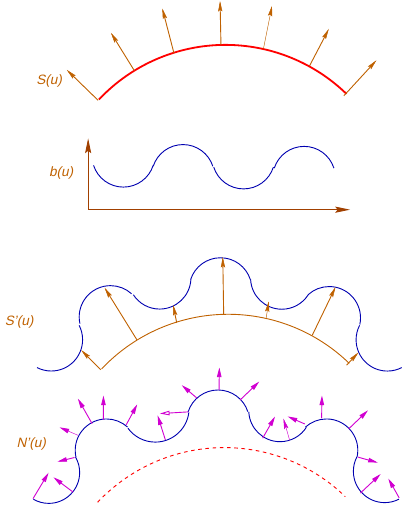
\includegraphics[width=5cm]{slike/03_bump_mapping.png}
			\end{center}
		\end{column}
		\begin{column}{7cm}
			\begin{center}
				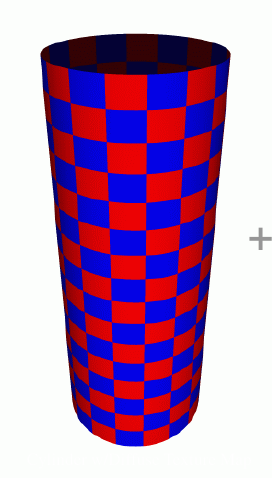
\includegraphics[width=1.8cm]{slike/bump_01.png}
				
\includegraphics[width=1.8cm]{slike/bump_02.png}
				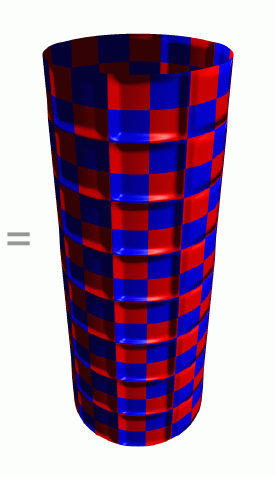
\includegraphics[width=1.8cm]{slike/bump_03.png}
			\end{center}
			\begin{center}
				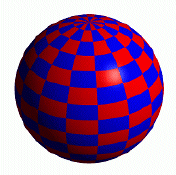
\includegraphics[width=1.8cm]{slike/bump_01_01.png}
				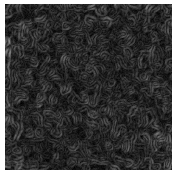
\includegraphics[width=1.8cm]{slike/bump_02_02.png}
				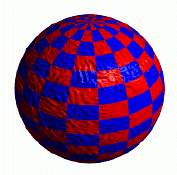
\includegraphics[width=1.8cm]{slike/bump_03_03.png}
			\end{center}
		\end{column}
	\end{columns}
\end{frame}
%
\begin{frame}{Displacement mapping}
	Vrijednosti teksture su vrijednosti pomaka geometrije u smjeru normale.
	\begin{center}
		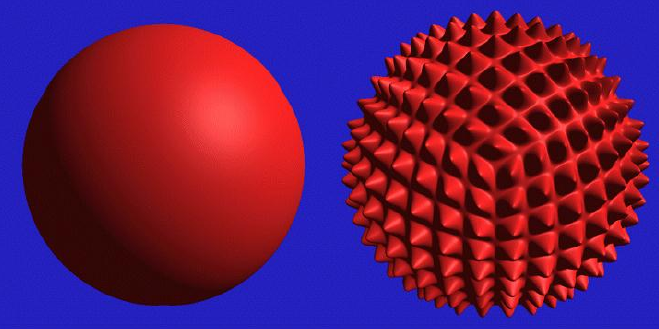
\includegraphics[width=2.5cm]{slike/displacement_map.png}
	\end{center}
	\begin{block}{}
		Bump mapping općenito ne zahtijeva puno resursa. Displacement mapping zahtijeva više resursa tijekom
		inicijalizacije i manipulacije, ali kako se računanje odvija tijekom postavljanja scene, ne povećava vrijeme renderiranja, dok bump mapping povećava vrijeme renderiranja iz razloga što pokreće novi shader proces.
	\end{block}
	
	
\end{frame}
%
%\begin{frame}{Bump vs Displacement mapping}
%	\begin{block}{Primjena Displacement mapping}
%		\begin{itemize}
%			\item tereni
%			\item animacija travnatih i šumovitih područja
%			\item valovi vodenih i sličnih površina
%			\item animacija vatre, dima, oblaka ili sličnih čestičnih volumena
%		\end{itemize}
%	\end{block}
%	
%	\begin{block}{Primjena Bump mapping}
%		\begin{itemize}
%			\item realizam tekstura - koža itd.
%			\item dodavanje malih detalja objektu
%		\end{itemize}
%	\end{block}
%\end{frame}
%
\begin{frame}{Bump vs Displacement mapping contd.}
	\begin{center}
		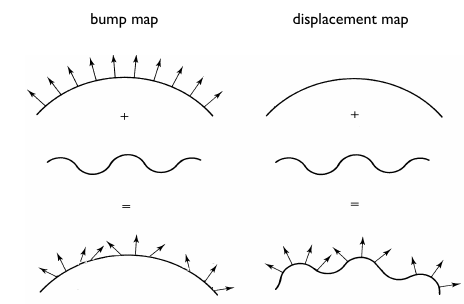
\includegraphics[width=10cm]{slike/03_bump_vs_displacement_mapping.png}
	\end{center}
\end{frame}

\begin{frame}{Bump vs Displacement mapping contd.}
	\begin{center}
		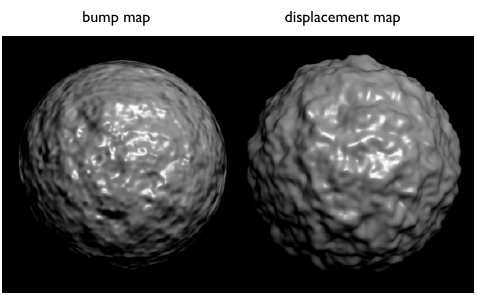
\includegraphics[width=10cm]{slike/03_bump_vs_displacement_mapping_a.png}
	\end{center}
\end{frame}

\begin{frame}{Bump/Normal mapping}
	Problem:
	\begin{center}
		
\includegraphics[width=8cm]{slike/normal_mapping_surfaces.png}
	\end{center}
	\begin{center}
	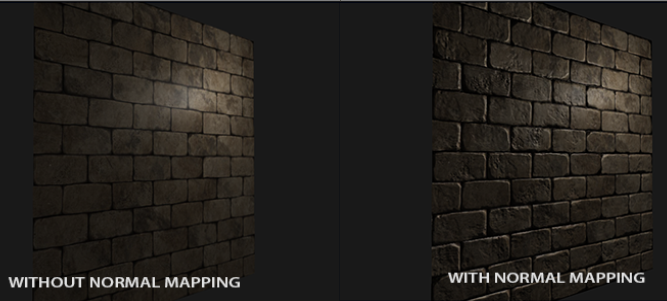
\includegraphics[width=11cm]{slike/normal_mapping_compare.png}
	\end{center}
\end{frame}

\begin{frame}{Normale}
	\begin{itemize}
		\item Boja: $(\mathrm{r}, \mathrm{g}, \mathrm{b})$
		\item Normala: $(x, y, z)$
		\item Normale možemo spremiti u sliku
		\item $x$ u $u$ smjeru, $y$ u $v$ smjeru, $z$ smjer: $u\times v$
	\end{itemize}
	
	\begin{center}
		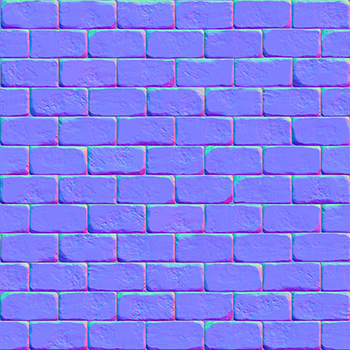
\includegraphics[width=4cm]{slike/normal_mapping_normal_map.png}
	\end{center}
\end{frame}
\begin{frame}{Još jedan problem}
	Normale iz teksture odgovaraju globalnom koordinatnom sustavu.
	
	\begin{center}
		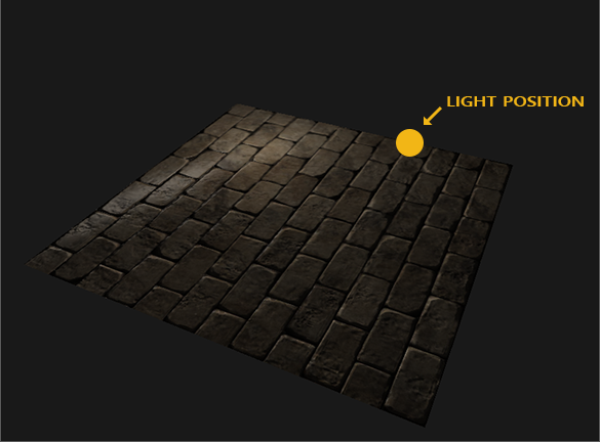
\includegraphics[width=4cm]{slike/normal_mapping_ground.png}
		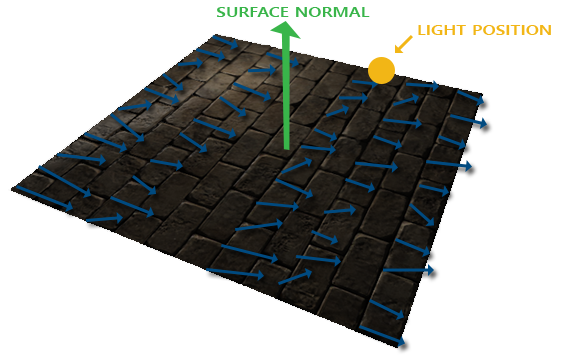
\includegraphics[width=5cm]{slike/normal_mapping_ground_normals.png}
	\end{center}
\end{frame}
\begin{frame}{Tangente i normala}

	\begin{columns}
		\begin{column}{0.7\textwidth}
			\begin{itemize}
				\item Koordinate verteksa: $P_1$,$P_2$ i $P_3$
				\item Znamo $(u, v)$ za svaki verteks, $P_1$,$P_2$ i $P_3$
				\item $E_1 = \Delta U_1 T +\Delta V_1 B$, $E_2 = \Delta U_2 T +\Delta V_2 B$
			\end{itemize}
			\begin{align*}
			(E_{1x}, E_{1y}, E_{1z}) = \Delta U_1(T_x, T_y, T_z) + \Delta V_1(B_x, B_y, B_z) \\
			(E_{2x}, E_{2y}, E_{2z}) = \Delta U_2(T_x, T_y, T_z) + \Delta V_2(B_x, B_y, B_z)
			\end{align*}
			ili
			\begin{align*}
			\begin{pmatrix}
				E_{1x} & E_{1y} & E_{1z} \\
				E_{2x} & E_{2y} & E_{2z}
			\end{pmatrix}
			=
			\begin{pmatrix}
			\Delta U_1 & \Delta V_1 \\
			\Delta U_2 & \Delta V_2
			\end{pmatrix} 
			\begin{pmatrix}
			T_x & T_y &  T_z \\
			B_x & B_y &  B_z
			\end{pmatrix} 
			\end{align*}
		\end{column}
		\begin{column}{0.3\textwidth}
				\begin{center}
				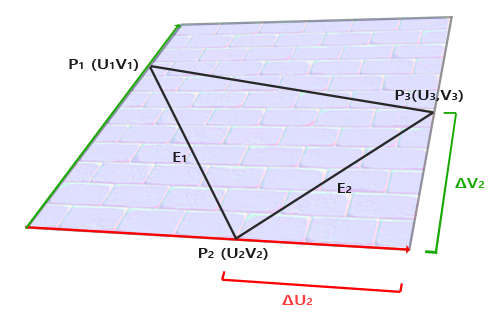
\includegraphics[width=3cm]{slike/normal_mapping_surface_edges.png}
			\end{center}
			\begin{center}
				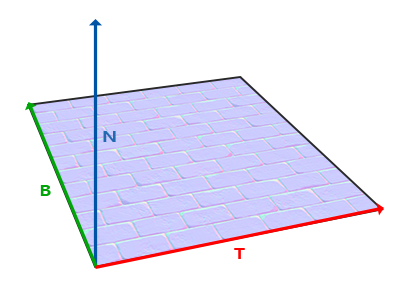
\includegraphics[width=3cm]{slike/normal_mapping_tbn_vectors.png}
			\end{center}
		\end{column}
	\end{columns}
	Na kraju dobijemo:
	\begin{align*}
	\begin{pmatrix}
	T_x & T_y &  T_z \\
	B_x & B_y &  B_z
	\end{pmatrix} = 
	\frac{1}{\Delta U_1\Delta V_2 - \Delta U_2\Delta V_1}
	\begin{pmatrix}
	\Delta V_2 & -\Delta V_1 \\
	-\Delta U_2 & \Delta U_1
	\end{pmatrix} 
	\begin{pmatrix}
	E_{1x} & E_{1y} & E_{1z} \\
	E_{2x} & E_{2y} & E_{2z}
	\end{pmatrix}
	\end{align*}
\end{frame}
\begin{frame}{Tangente i normala, contd.}
	\begin{align*}
	T_x = \frac{1}{\Delta U_1\Delta V_2 - \Delta U_2\Delta V_1} (\Delta V_2 E_{1x}-\Delta V_1 E_{2x}) \\
	T_y = \frac{1}{\Delta U_1\Delta V_2 - \Delta U_2\Delta V_1} (\Delta V_2 E_{1y}-\Delta V_1 E_{2y}) \\
	T_z = \frac{1}{\Delta U_1\Delta V_2 - \Delta U_2\Delta V_1} (\Delta V_2 E_{1z}-\Delta V_1 E_{2z})
	\end{align*}
	
	$B$ se može izračunati i ovako:
	\begin{align*}
	B = N \times T
	\end{align*}
\end{frame}
\begin{frame}{Displacement mapping}
	content...
\end{frame}
\plain{Pitanja?}
\end{document}